%*******************************************************************************
%****************************** Third Chapter *********************************
%*******************************************************************************

\chapter{Inhomogeneous Electroluminescence in InGaN QW LEDs}

\ifpdf
    \graphicspath{{Chapter2/Figs/Raster/}{Chapter2/Figs/PDF/}{Chapter2/Figs/}}
\else
    \graphicspath{{Chapter2/Figs/Vector/}{Chapter2/Figs/}}
\fi


\section[Short title]{Background}

% Uncomment this line, when you have siunitx package loaded.
%The SI Units for dynamic viscosity is \si{\newton\second\per\metre\squared}.

$\mathrm{In_{x}Ga_{1-x}N}$/GaN QW structures are key structures in present day light emitting diodes in the visible wavelengths. Despite the growth of III-nitride LEDs into a gigantic market with a projected overall worth of 64 billion EUR by 2020, III-nitride alloys suffer from a plethora of material issues arising from heteroepitaxial growth on foreign substrates with large lattice mismatches \cite{Bennett2010b}. A notorious issue in III-nitride growth is the high density of threading dislocations which are the source of highly undesirable effects in diode structures such as non-radiative recombination \cite{Albrecht2008} and leakage current \cite{Bennett2010b}.\\
Threading dislocations have been shown to result in inverted pyramidal defects at the surface of nitride epilayers, known as 'V defects'. The effect of these defects on LED performance is hotly debated in literature as they are expected by many to hinder LED performance due to their association with TDs. However, it has been shown that narrower QWs along the sidewalls of V-defects serve to screen carriers from the non-radiative centres at TDs \cite{Hangleiter2005}.\\
In this study, a 'multi-microscopy' approach whereby several microscopy techniques are utilised on the same features is used to elucidate the origin of inhomogeneous EL in $\mathrm{In_{x}Ga_{1-x}N}$/GaN QW structures. The correlation of emissive and structural properties at the surface of the LED structures using several microscopy techniques has allowed for the detection of hexagonal defects at the centre of the inhomogeneities. Following this, structural and compositional information obtained using this combination of techniques is then used to simulate and reproduce the inhomogeneous EL, thus elucidating the mechanism whereby hexagonal defects can cause inhomogeneous EL in LEDs.


\section{Sample Structure}
For this study, two multiple QW InGaN LED structures of different QW nominal thicknesses (3.5 nm and 4.5 nm) were studied. Both samples were grown at the Cambridge Centre for Gallium Nitride, with LED processing carried out at the University of Bath. The structures were grown on low dislocation density \nomenclature[z-LDD]{LDD}{Low Dislocation Density} ($5 \times 10^{8}cm^{-2}$) GaN template on sapphire, and consist of a 2 $\mu m$ layer of unintentionally doped GaN followed by a 3 $\mu m$ silicon doped GaN layer. The active layer consists of a 5 period InGaN/GaN MQW region, with unintentionally doped GaN barriers (7.6 nm). An AlGaN electron blocking layer \nomenclature[z-EBL]{EBL}{Electron Blocking Layer} (20 nm) and a magnesium-doped GaN cap (117 nm) were grown following the active region. This is shown schematically in Fig. \ref{LEDstruct}:

\begin{figure}[!ht]
	\centering
	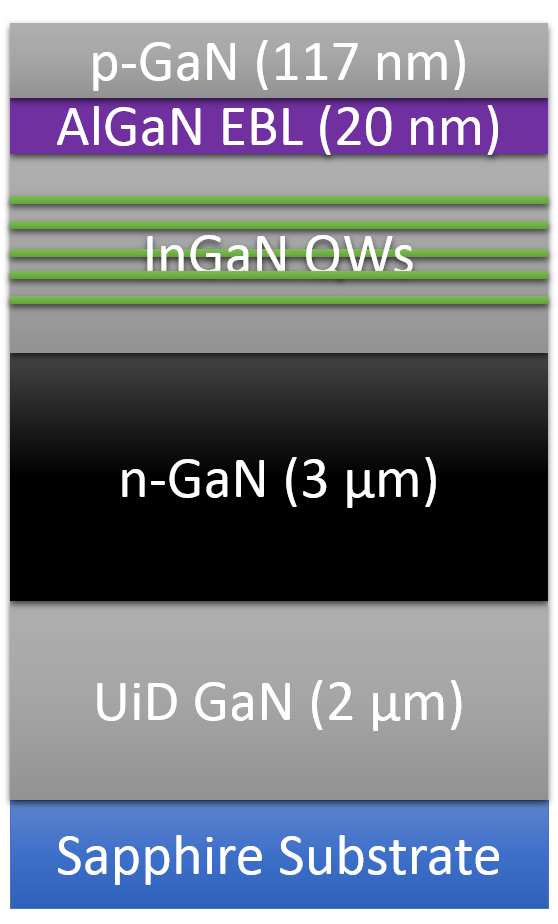
\includegraphics[width=0.4\textwidth]{Figs/Ch3/LEDstruct}
	\caption[h] {LED structure schematic.}
	\label{LEDstruct}
\end{figure}

\FloatBarrier 
The wafers were processed into $1 \times 1 mm^{2}$ side contacted LEDs with thin oxidized Ni/Au current spreading {\it p}-layer Ohmic contact. Ti/Al Ohmic contact stripes were deposited on the {\it n}-layer and the Ni/Au current spreading layer in an interdigitated geometry.\\
QW thickness for both samples was determined from X-ray diffraction \nomenclature[z-XRD]{XRD}{X-ray Diffraction} (XRD) using the method described by Vickers {\it et al.} \cite{Vickers2003}. The QWs were grown using the '2T' method, whereby the growth temperature is ramped up immediately following the InGaN growth under ammonia but without metalorganic fluxes. The barrier growth begins towards the end of the temperature ramp, this typically leads to loss of indium during the temperature ramp which can cause gross well-width fluctuations \cite{Laak2013} but a higher barrier growth temperature is preferable\cite{Oliver2013}. '2T' growth is shown schematically in Fig.\ref{2T}.

\begin{figure}[!ht]
	\centering
	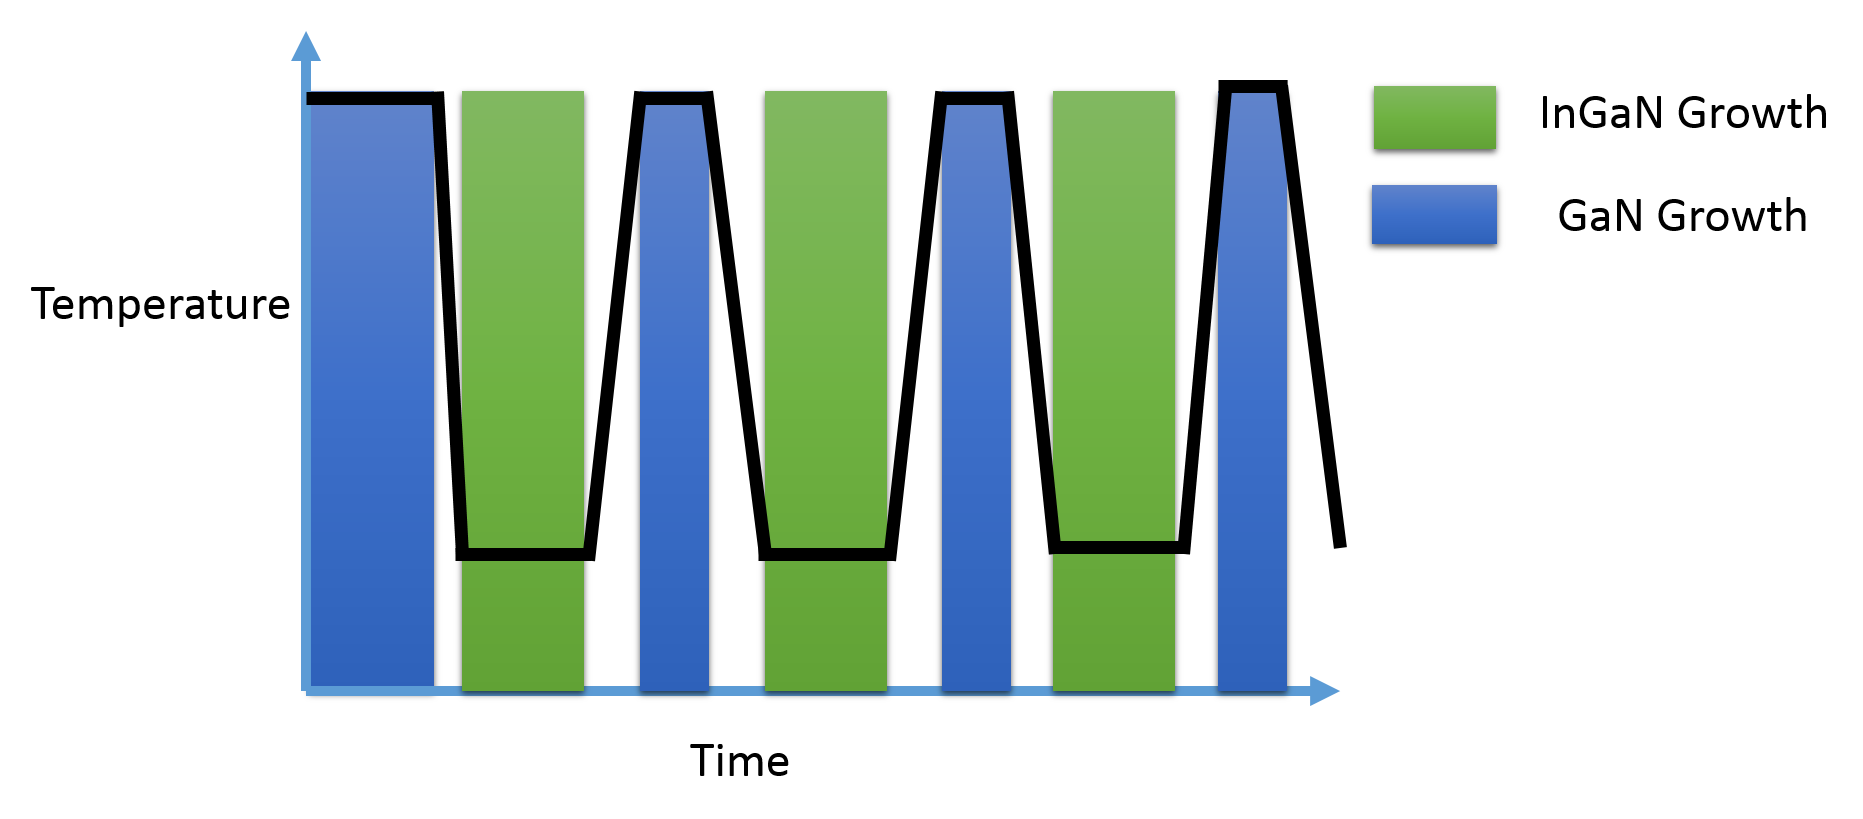
\includegraphics[width=0.9\textwidth]{Figs/Ch3/2T}
	\caption[h] {'2T' growth of InGaN/GaN QWs. GaN QB growth is halted during the temperature ramp. The black trace indicates growth temperature over time.}
	\label{2T}
\end{figure}

\FloatBarrier 

\section{Experimental}

Initial evaluation of the inhomogeneous EL was performed in a Signatone S-1160 probe station under forward bias, as shown in Fig.\ref{probe}.

\begin{figure}[h]
	\begin{subfigure}[t]{0.35\textwidth}
		\centering
		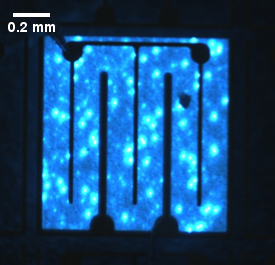
\includegraphics[width = 1\textwidth]{Figs/Ch3/5610.png}
		\caption{}
	\end{subfigure}%
	\hspace*{2cm}
	~	
	\begin{subfigure}[t]{0.35\textwidth}
		\centering
		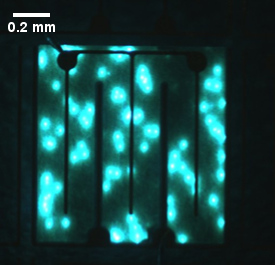
\includegraphics[width=1\textwidth]{Figs/Ch3/5608.png}
		\caption{}
	\end{subfigure}
	\caption {a) C5610A b) C5608A EL under a forward bias of 3V. The bright inhomogeneities are visible in the emission of the LEDs. }
	\label{probe}
\end{figure}
\FloatBarrier


Following this, hyperspectral EL mapping with CL and EBIC were performed using a modified Cameca SX100 electron probe micro-analyser with a custom built cathodoluminescence set-up. Hyperspectral EL measurements were performed under forward bias, enabling the acquisition spatially resolved EL maps of the inhomogeneities. Following the detection of hexagonal defects at the centre of inhomogeneities using SEM-CL, the defects were analyzed using AFM and C-AFM. Finally, FIB/SEM lamella preparation techniques were used to perform HAADF-STEM and STEM-EDX on the defects, allowing for access nanoscale compositional and structural information required to reproduce the EL in simulations.


\subsection{Hyperspectral EL Imaging}
Hyperspectral EL imaging was performed at Strathclyde University with the assistance of Dr Michael Wallace. In order to study the device under forward current, the LED wafers were mounted on TO-5 headers and bonded with 5 µm Al wire. A Keithley Instrument 2401 source meter was used to apply varying forward currents to the devices and thus allow for the collection of EL. \\
Full EL spectra were collected with a spatial resolution of approximately 3 µm and analysed using custom software developed by Dr. Paul Edwards, allowing for 2-D maps of EL peak intensity, position and FWHM. At each pixel in the map, a full EL spectrum was collected by an Andor CCD camera. A full set of data extracted from the hyperspectral EL mapping is shown in Fig.\ref{ELfull}

\begin{figure}[!ht]
	\centering
	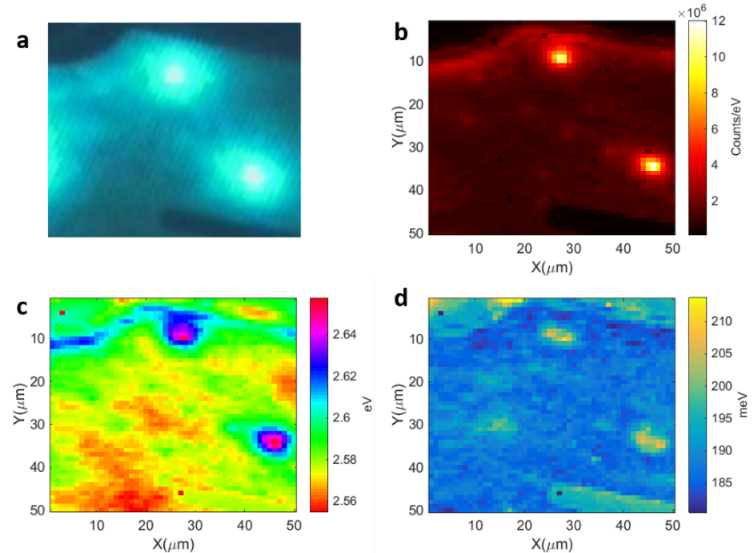
\includegraphics[width=0.8\textwidth]{Figs/Ch3/ELfull}
	\caption[h] {a) Probe station image b) EL peak intensity, c) EL peak energy and d) EL FWHM extracted by fitting the hyperspectral EL data under a forward current of 10 mA}
	\label{ELfull}
\end{figure}

\FloatBarrier 

It is interesting to note that from this representative data set, the inhomogeneities observed are brighter by a factor of $\sim 6$, blue-shifted in terms of peak energy by $\sim 0.08$ eV and have a larger FWHM. Although these values were observed to shift based on injection current, the overall trend observed in all data sets for both LED devices is represented by Fig.\ref{ELfull}.

\subsubsection{Current Dependent EL Measurements}

\begin{figure}
	\begin{subfigure}[b]{0.48\textwidth}
		\centering
		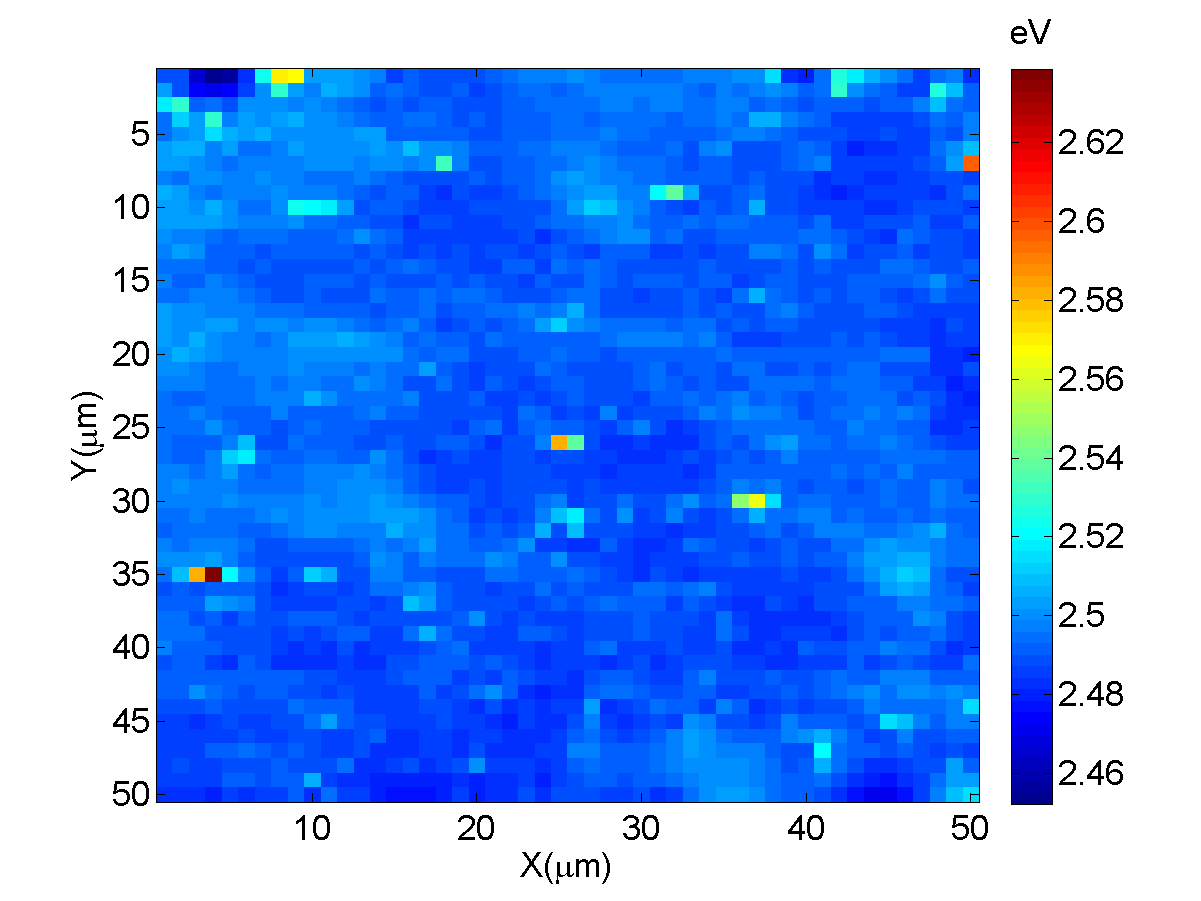
\includegraphics[width=1\linewidth]{Figs/Ch3/1}
		\caption{1 mA}
	\end{subfigure}%
	\hspace*\fill
	\begin{subfigure}[b]{0.48\textwidth}
		\centering
		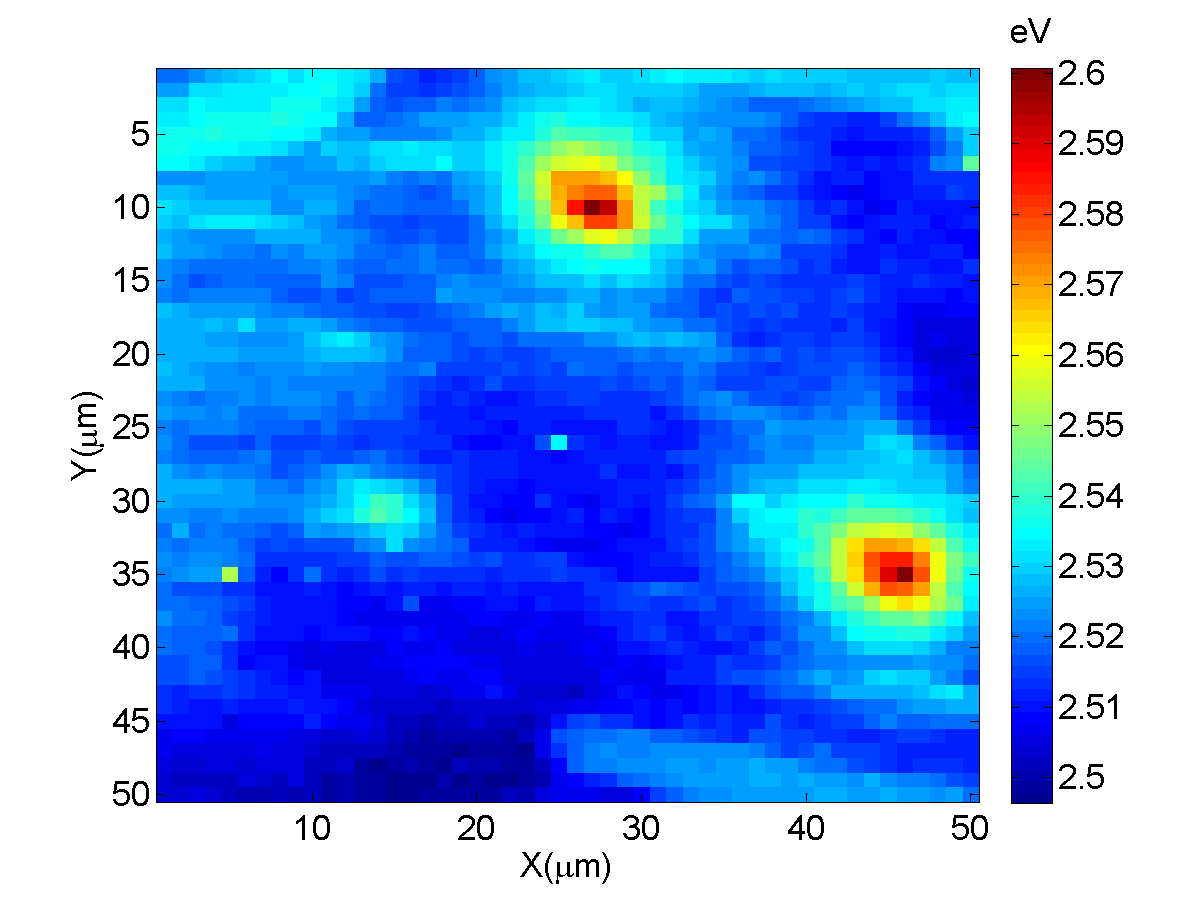
\includegraphics[width=1\linewidth]{Figs/Ch3/5}
		\caption{5 mA}		
	\end{subfigure}%
	
	\medskip
	\begin{subfigure}[b]{0.48\textwidth}
		\centering
		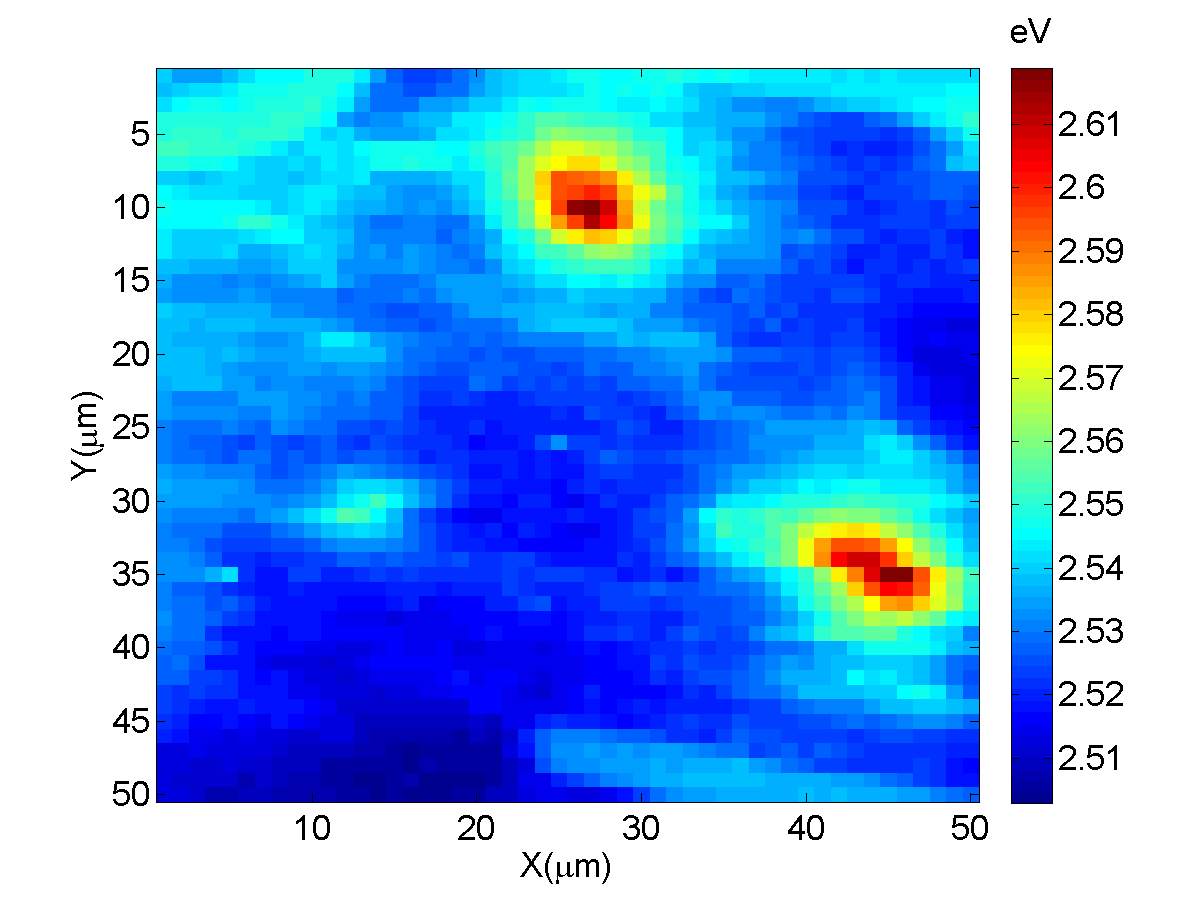
\includegraphics[width=1\linewidth]{Figs/Ch3/10}
		\caption{10 mA}
	\end{subfigure}%
	\hspace*\fill
	\begin{subfigure}[b]{0.48\textwidth}
		\centering
		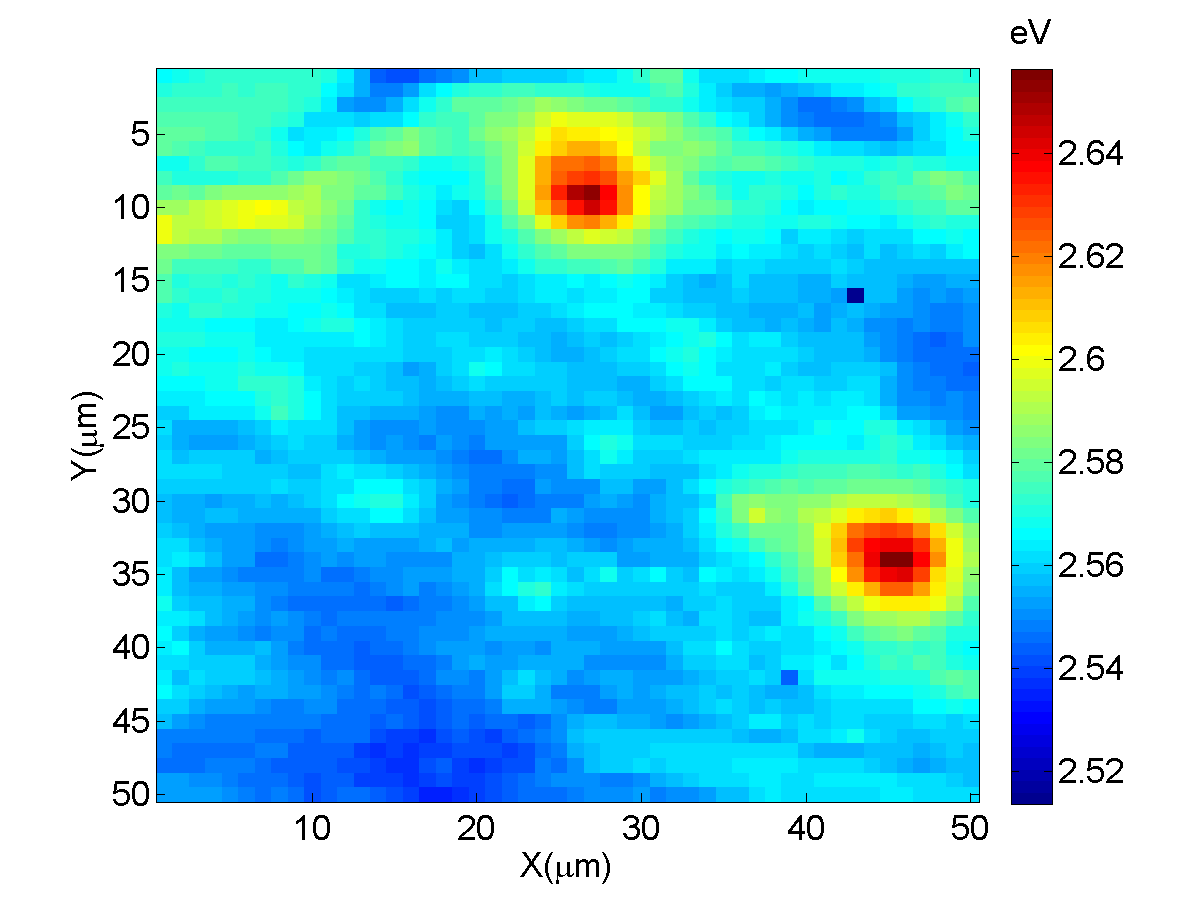
\includegraphics[width=1\linewidth]{Figs/Ch3/50}
		\caption{50 mA}		
	\end{subfigure}%
	
	\medskip
	\begin{subfigure}[b]{0.48\textwidth}
		\centering
		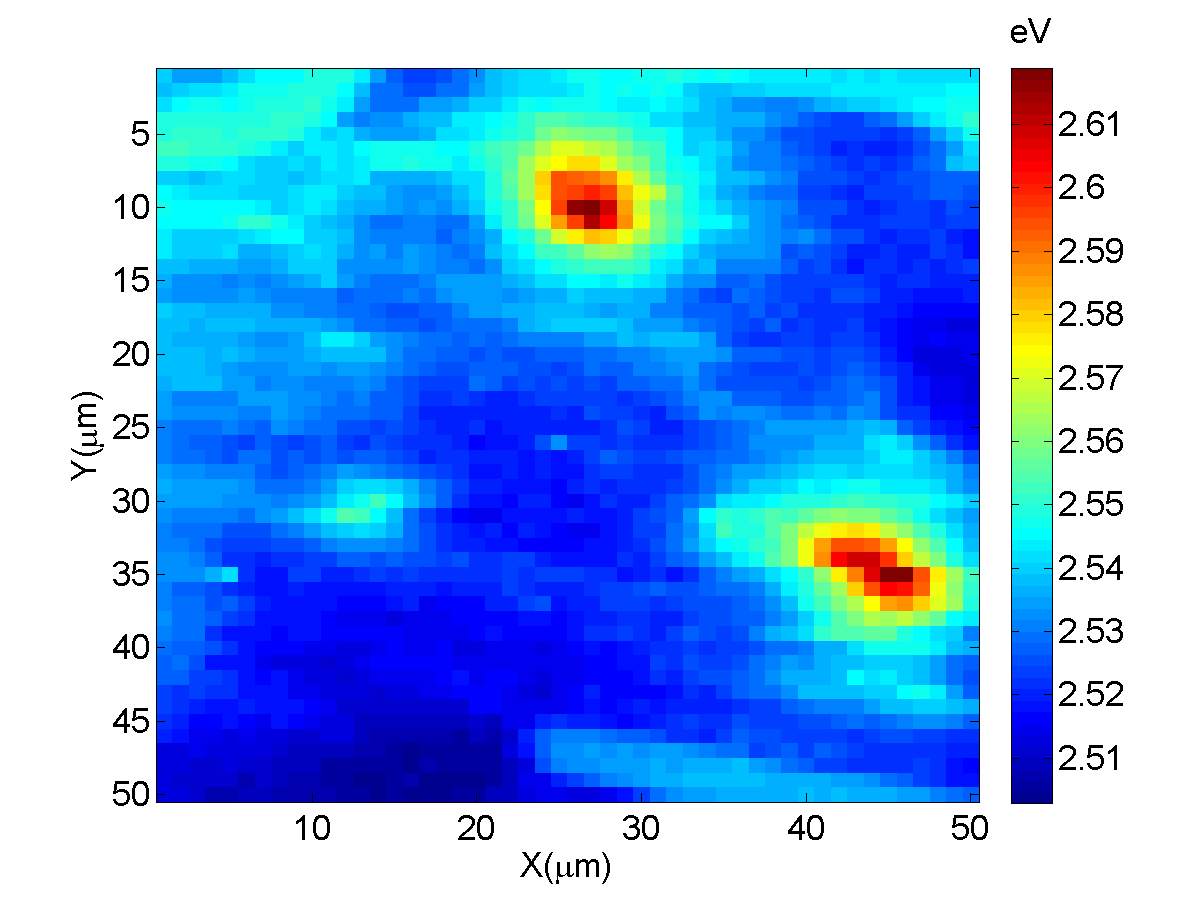
\includegraphics[width=1\linewidth]{Figs/Ch3/10}
		\caption{10 mA}
	\end{subfigure}%
	\hspace*\fill
	\begin{subfigure}[b]{0.48\textwidth}
		\centering
		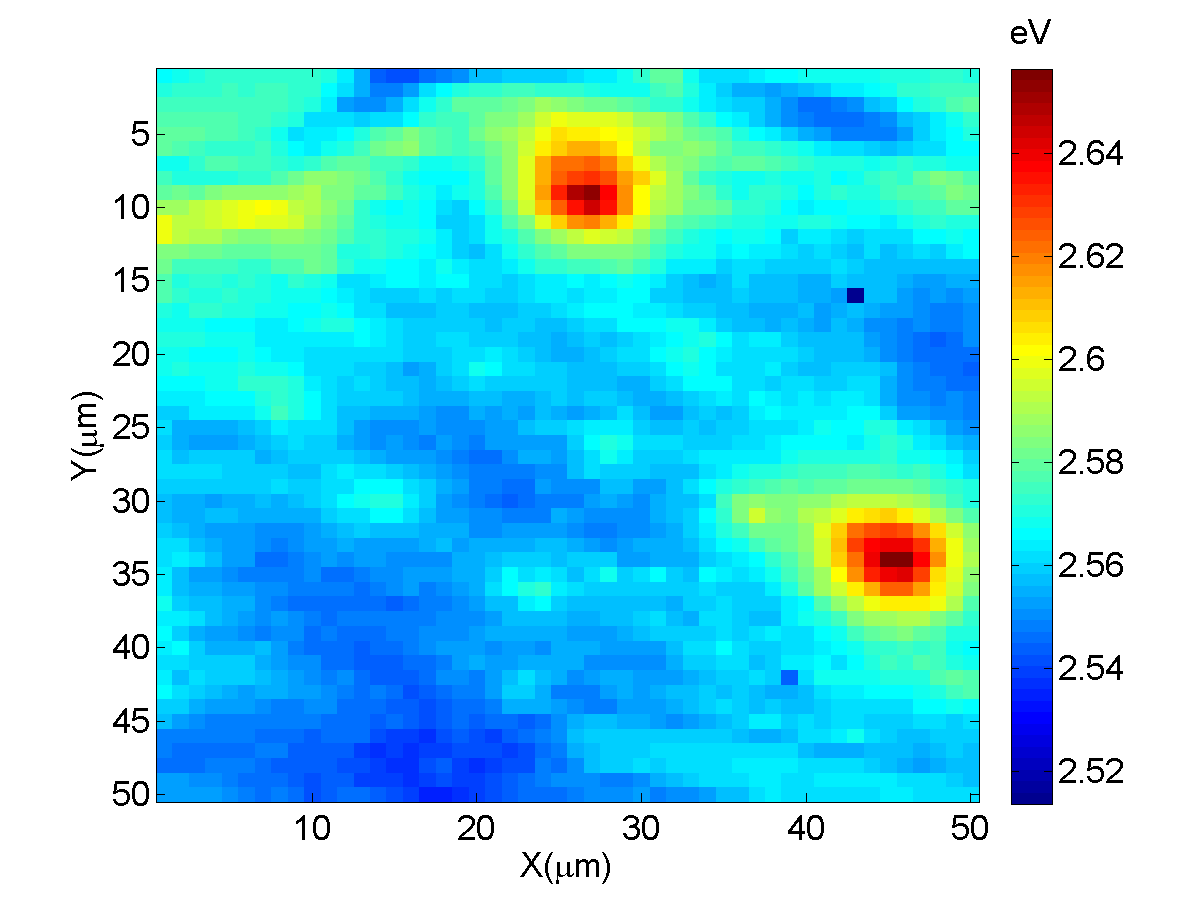
\includegraphics[width=1\linewidth]{Figs/Ch3/50}
		\caption{50 mA}		
	\end{subfigure}%
	
	\caption{Peak Intensity for Varying Current}
	\label{peak5610}
\end{figure}

\FloatBarrier
\subsection{Cathodoluminescence and Electron Beam Induced Current}
CL and EBIC images showing rings + CL/SEM showing pits.

\subsection{Hexagonal Defect Analysis}

\subsection{Scanning Electron Microscopy}

\subsection{Atomic Force Microscopy}
AFM images of pits + C-AFM
\subsubsection{Conductive-AFM}

\subsection{TEM Lamella preparation}

\subsection{Scanning Transmission Electron Microscopy}
\subsubsection{Hexagonal Defect Morphology}
\subsubsection{Compositional Analysis}

\section{Simulations}

\section{Conclusion}

\section{Future Work}

